\documentclass[10pt]{article}
\usepackage[letterpaper,margin=0.72in]{geometry}
\usepackage{graphicx}
\usepackage{booktabs}
\usepackage[T1]{fontenc}
\usepackage{hyperref}
\hypersetup{pdftitle={Finite Frobenius certificate for the archived BINSTD field}}
\setlength{\parindent}{0pt}
\setlength{\parskip}{0.43em}
\begin{document}
\begin{center}
{\Large\bfseries Finite Frobenius certificate for the archived BINSTD field}\\[0.35em]
27 October 2026 \quad $\mathrm{EXP}$-BINSTD-8bdf86 \quad source commit \texttt{c03b34d71c}
\end{center}

\textbf{Scope.} Deterministic code and finite-algebra audit of the frozen $n=17$ bitmask field helper. It changes no archived run, research decision, Lean theorem status, or performance estimate. The helper's SHA-256 matches the archived run source map: \texttt{402cf41f4d52\ldots b668c8b3d955}.

\textbf{Finite checks.} An independent bit-position squaring and polynomial remainder implementation agrees with the archived \texttt{Field.sqr} and its $\mathbf F_2$ matrix action for all $2^{17}=131{,}072$ field values. Trial division finds no monic proper divisor of $t^{17}+t^3+1$ in degrees 1--8 among 510 candidates. The resulting Frobenius matrix has order 17. Bitmask 3 has a 17-element Frobenius orbit of rank 17, supplying a concrete cyclic/normal-basis witness.

The checked factor bitmasks $3$, $313$, $471$ multiply to $X^{17}+1$ and are individually irreducible. Their concrete matrix kernels have dimensions $1$, $8$, $8$. The degree subset sums are $\{0,1,8,9,16,17\}$, matching the archived table. The figure below displays these finite values; bar widths are dimensions, not speed measurements.

\textbf{Formal boundary.} The finite witness gives premises for the cyclic-module interpretation, but the runner-to-canonical field map and the theorem that \emph{every} invariant subspace arises from the three factors are still open in Lean. This Python audit does not prove empirical yield, target independence, runtime advantage, attack cost, or security impact. The source-bound factor and canonical Frobenius Lean results in PR \#2484 retain their narrower statements and still need independent semantic review.

\textbf{Reproduction.} Run the audit on the pinned commit and compare its JSON with the archived certificate. Normal and optimized Python produced byte-identical outputs. Exact commands, full hashes, source, method, and limitations are in the accompanying Markdown report.

\vspace{1.3em}
\begin{center}
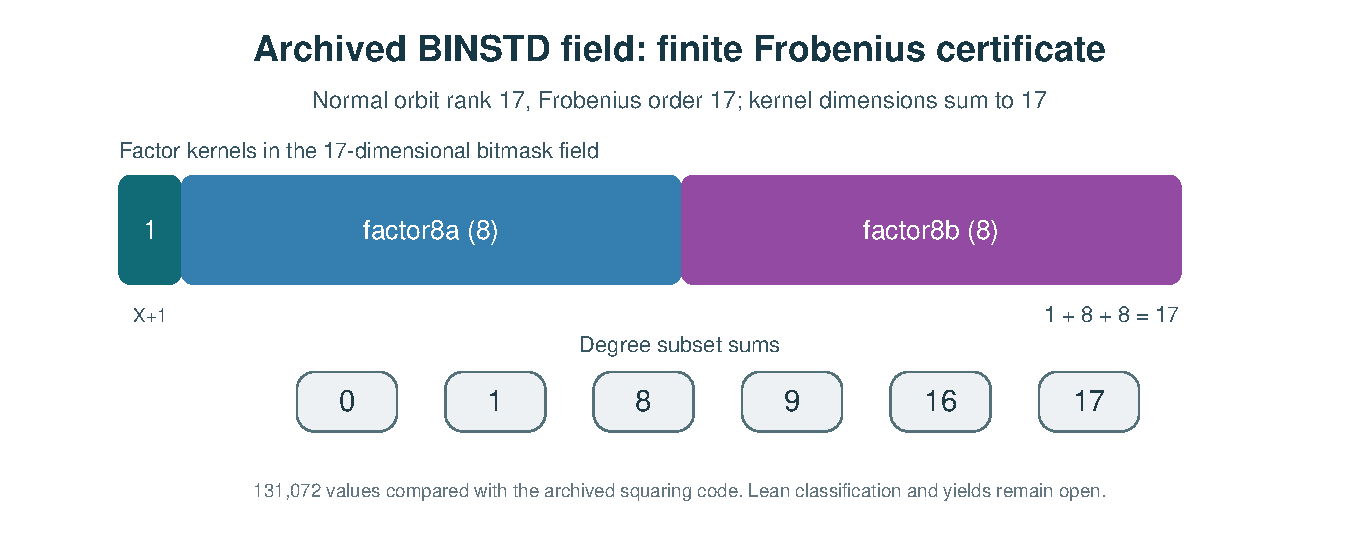
\includegraphics[width=\textwidth,height=0.32\textheight,keepaspectratio]{factor-kernels-figure.pdf}
\end{center}
\end{document}
